\section*{Appendix A: Comparison and analysis of the bisimulation equivalence algorithms}
\label{appendixA}

There is no official set of benchmarks for testing algorithms for computing bisimulation equivalence \cite{PiazzaPolicriti}. And it is also very difficult to randomly generate labeled transition systems suitable for proper testing of bisimulation equivalence. Therefore, we used the academical examples from mCRL2 as experimental test models. 

The experiments were conducted on a portable computer with the following specifications: 
\begin{enumerate}
	\item CPU: Intel Pentium P6100 2.0 GHz
	\item Memory: 3 GB
	\item OS: Windows 2007 Premium
\end{enumerate}

The experiments carried out on our Java implementations of the two algorithms for computing strong bisimilarity consisted of 10 repeated runs of each of the algorithms for each of the Aldebaran test files. average running time in miliseconds. 
The results from these experiments are presented in Table~\ref{table2}. The table includes the running times and the absolute error in miliseconds for both of the algorithms, the number of bisimilar pairs obtained with the naive algorithm (excluding the reflexive and symmetric pairs) and the number bisimilar equivalence classes obtained with the algorithm due to Fernandez (excluding the one-element classes), as well as the ratio of the running time of the naive algorithm with respect to the running time of Fernandez's algorithm.

\begin{table}
\begin{tabular}{| l | l | l | l | l | l | l | p{1.3cm}  | p{1.3cm} | l | }

	\hline 
	\multicolumn{3}{|c} { }
	& \multicolumn{2}{|c|}{Naive}
	& \multicolumn{2}{|c|}{Fernandez}
	& \multicolumn{2}{|c|} { }
	& Ratio
	\\ \hline  
  \hline                       
	aut &
	states &
	transitions &
	$t(ms)$ &
	$\Delta t(ms)$ &
	$t(ms)$ &
	$\Delta t(ms)$ &
	bisimilar pairs &
	bisimilar classes &
	$t_{n}/t_{f}$
	\\ \hline
	
	dining3 &
	93 &
	431 &
	16.8 &
	0.8 &
	250 &
	2 &
	1 &
	2 &     
	0.067
	\\ \hline
	
	abpbw &
    97 &
    122 &
    287.9 &
    0.94 &
    173.3 &
    5.22 &
    32 &
    27 &
    1.661   
    \\ \hline
	
	abp &
    74 &
    92 &
    162.2 &
    1.44 &
    69.6 &
    3.92 &
    6 &
    6 &
    2.33   
    \\ \hline
	
	scheduler &
	13 &
	19 &
	17.4 &
	1.18 &
	4.4 &
	0.96 &
	1 &
	1 &
	3.95   
	\\ \hline
	
	mpsu &
	52 &
	150 &
	215.4 &
	1.16 &
	27.5 &
	0.5 &
	4 &
	4 &
	7.83   
	\\ \hline
  
    trains &
    32 &
    52 &
    64.5 &
    7.3 &
    7.6 &
    1.76 &
    6 &
    6 &
    8.48   
    \\ \hline
	
    par &
    94 &
    121 &
    5909.4 &
    22.68 &
    28.5 &
    0.7 &
    170 &
    27 &
    207.34   
    \\ \hline  
  
    leader &
    392 &
    1128 &
    / &
    / &
    841.5 &
    41.5 &
    / &
    20 &
    /   
    \\ \hline
  
    tree &
    1025 &
    1024 &
    / &
    / &
    1858.1 &
    55.16 &
    / &
    8 &     
    / \\ \hline 
  
    cabp &
    672 &
    2352 &
    / &
    / &
    16184.3 &
    198.94 &
    / &
    90 &     
    /
   \\ \hline
  
\end{tabular}
\caption{Results of the comperisons}
\label{table2}
\end{table}
These experimental results are presented graphically in Fig.~\ref{fig:naiveAnalysis} and Fig.~ \ref{fig:fernandezAnalysis} for the naive algorithm and the algorithm of Fernandez, respectively. 

\begin{figure}[h]
\centering
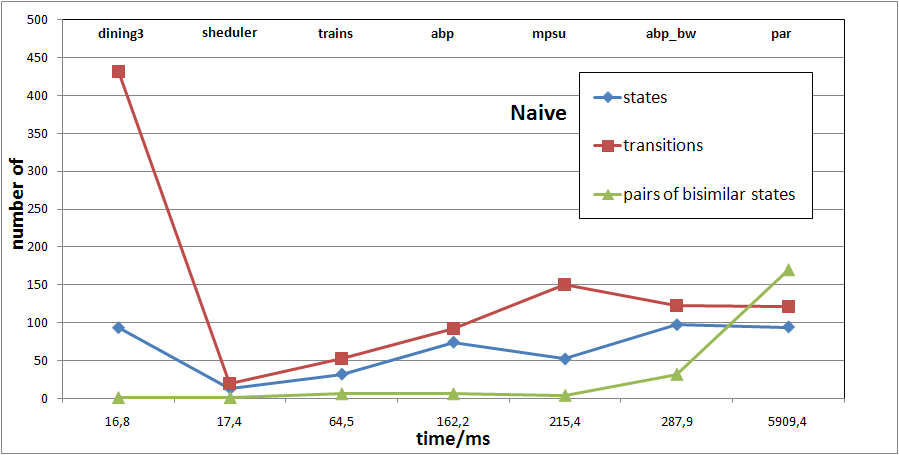
\includegraphics[width=5.0in]{naive}
\caption{Analysis of the running time of the naive bisimulation algorithm}
\label{fig:naiveAnalysis}
\end{figure}

\begin{figure}[h]
\centering
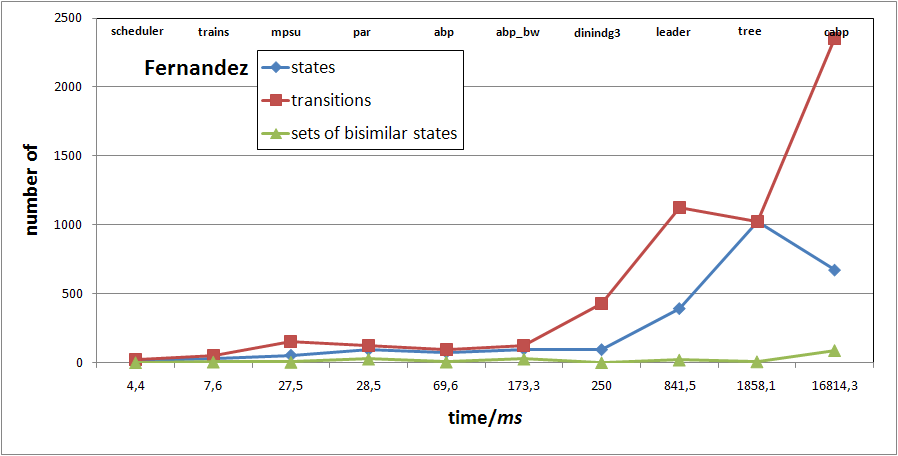
\includegraphics[width=5.0in]{fernandez}
\caption{Analysis of the running time of the bisimulation algorithm due to Fernandez}
\label{fig:fernandezAnalysis}
\end{figure}

As it can be easily seen, for all test models, with the exception of the first one, the running time of the naive algorithm is proportional to the number of states, the number of transitions and the number of resulting bisimilar pairs. However, we need to note that this is not a general conclusion. In general the running time of the naive algorithm for computing bisimulation equivalence depends on the nature of the monotonic function used by this algorithm, which is strongly related with the form of the labeled transition system. As an example, dining3.aut is a labeled transition system that has a big number of transitions, however in this test model the algorithm determines that the monotony condition is not fulfilled already in the second development of the monotonic function and therefore the algorithm stops there.

Similar conclusions can be drawn for the algorithm due to Fernandez. Its running time is also proportional to the number of transitions, number of states and the number of bisimilar classes. 

The comparison of running times of the two algorithms obtained with the experiment is shown in Fig.~\ref{fig:comparison1}. As it can be clearly seen the algorithm of Fernandez is few times faster than the naive algorithm. The biggest difference can be noticed for the example par.aut where the ratio of the running times is 207.34. An exception is only the example dining3.aut for which the naive algorithm performs faster due to the reasons described earlier. The ratio of the running times in this case is 0.0067. Fig.~ \ref{fig:comparison2} shows the ratios of the running times of the two algorithms for each of the examples.

\begin{figure}[h]
\centering
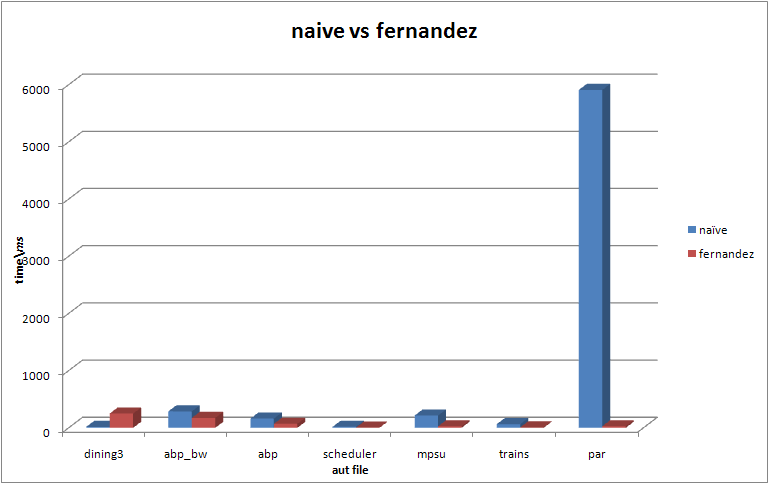
\includegraphics[width=5.0in]{compare1}
\caption{Comparison of the running times of the two bisimulation algorithms}
\label{fig:comparison1}
\end{figure}

\begin{figure}[h]
\centering
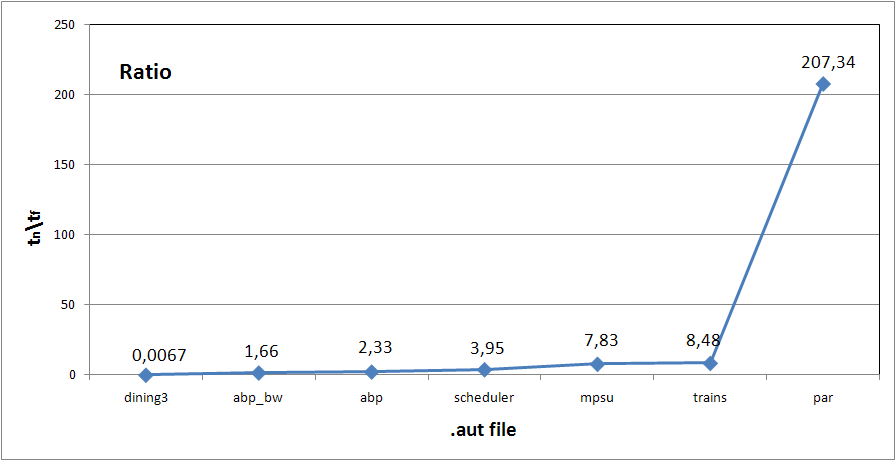
\includegraphics[width=5.0in]{compare2}
\caption{Ratio of the running times of the two bisimulation algorithms}
\label{fig:comparison2}
\end{figure}